\chapter{Reihenfolge-Kombinationen}

\section*{Lösung}

\begin{itemize}
    \item Preorder- und Inorder-Reihenfolge
    \item Postorder- und Inorder-Reihenfolge
\end{itemize}


\section*{Anmerkungen und Ergänzungen}

Zwei unterschiedliche Bäume seien wie in Abbildung~\ref{fig:AB} gegeben, wobei der linke Baum den Knoten $B$ als linken
Nachfolger hat, der rechte Baum den gleichen Knoten als rechten Nachfolger.
Die Preorder-Darstellung beider Bäume lautet $AB$, die Postorder-Darstellung lautet $BA$.
Folglich lässt sich nicht jeder binäre Baum allein durch die Kenntnis seiner Pre- und Postorder-Darstellung \textit{eindeutig} rekonstruieren.

\begin{figure}[h]
    \centering
    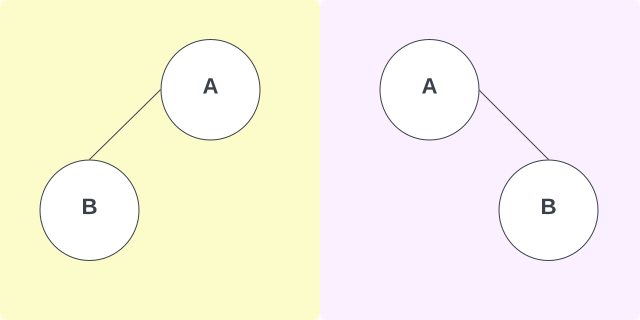
\includegraphics[
        width=10cm,
        keepaspectratio,
    ]{chapters/5. Reihenfolge-Kombinationen/img/AB}
    \caption{Beide Bäume besitzen die Preorder-Darstellung $AB$ und die Postorder-Darstellung $BA$, eine eindeutige Rekonstruktion ist nicht möglich.}
    \label{fig:AB}
\end{figure}

\textit{Knuth} weist in \cite[564]{Knu97} darauf hin, das sich ein \textit{vollständiger Baum}\footnote{
    Zur Definition ``vollständiger Baum`` siehe Abschnitt~\ref{ch:binprops}.
} tatsächlich durch seine Pre- und Postorder-Darstellung rekonstruieren läßt ({s. a.} Abbildungen~\ref{fig:ABC_pre}, ~\ref{fig:ABC_post} und~\ref{fig:ABC_complete})\footnote{
    ``If all nonterminal nodes of a binary tree have \textit{both} branches are nonempty, its structure \textit{is} characterized by preorder and postorder.``~\cite[564, 7., Hervorhebungen i.O.]{Knu97}
}.
Ebenda zeigt er, dass Pre- oder Postorder zusammen mit Inorder ausreichen, um einen binären Baum eindeutig zu rekonstruieren.

\blockquote[{\cite[564, 7.]{Knu97}}]{
   From the preorder, the root is known; then from the inorder, we know the left subtree and the right subtree; and in fact we know the preorder and inorder of the nodes in the latter subtrees. [...] Similarly, postorder and inorder together characterize the structure.
}\\


\begin{figure}[h]
\centering
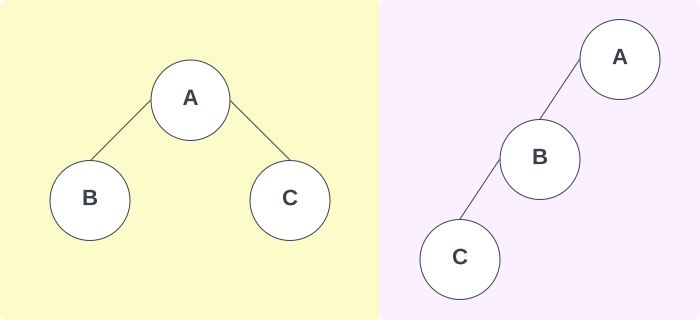
\includegraphics[
    width=10cm,
    keepaspectratio,
]{chapters/5. Reihenfolge-Kombinationen/img/ABC_pre}
\caption{Auch für einen vollständigen Baum (links) reicht seine Preorder-Darstellung zur eindeutigen Rekonstruktion nicht aus. Der Baum auf der rechten Seite besitzt dieselbe Preorder-Reihenfolge ($ABC$).}
\label{fig:ABC_pre}
\end{figure}

\begin{figure}[h]
\centering
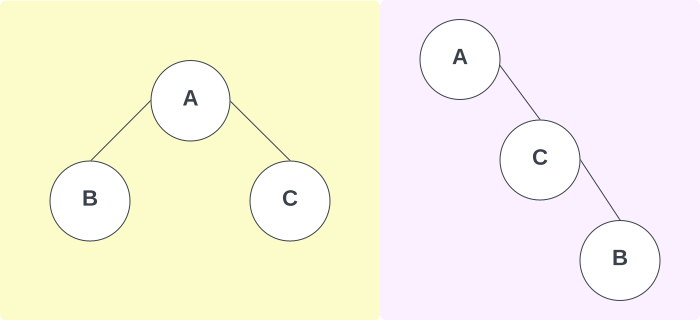
\includegraphics[
    width=10cm,
    keepaspectratio,
]{chapters/5. Reihenfolge-Kombinationen/img/ABC_post}
\caption{Der vollständige Baum (links) mit der Postorder-Darstellung $BCA$ und sein Pendant mit derselben Postorder-Reihenfolge.}
\label{fig:ABC_post}
\end{figure}

\begin{figure}[h]
\centering
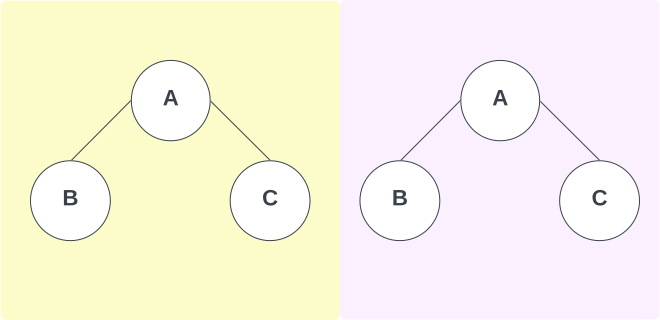
\includegraphics[
    width=10cm,
    keepaspectratio,
]{chapters/5. Reihenfolge-Kombinationen/img/ABC_complete}
\caption{Mit der Kenntnis von Pre- \textbf{und} Postorder-Reihenfolge ($ABC$ und $BCA$) lässt sich ein \underline{vollständiger} Baum eindeutig rekonstruieren.}
\label{fig:ABC_complete}
\end{figure}

Weitere Ausführungen zur Rekonstruktion von Binärbäumen finden sich bspw. bei \textit{Cameron, Bhattacharya und Merks}~\cite{CBM89}.
